% Drawing 141/01-2 -- folder 141, batch 01, archive page 9 (PDF page 10).
% Transcription: à gauche de « $\omega_1, \omega_2$, $\omega_2/\omega_1 = \tau$ », une sphère couverte de hachures obliques : contour rond, équateur en ellipse, trois gros points, un en haut et un en bas sur le contour, un sur l'arc avant de l'équateur.
% Kind: sphere covered with oblique hatching, three marked points. Method 2 (schematic redraw from the facsimile). Status: ok.
% Notes: As on the page, overlaid on the 400 dpi colour crop and redrawn 2026-11-12 (Opus 5.5): the outline is three strokes, not a round circle (an upper arc from the left through the top point to the right, a left lower arc and a right lower arc ending at the bottom point); the equator is a heavy back arc and a front arc that begins as the upper left part of the outline and runs through the front point to the right side; the hatching is one zigzag stroke of six legs, drawn as he drew it (from beyond the top point down to the left, up to the upper right, down to the lower left, up to the right, down to the lower left, back to the right along a curve, and a short leg down). Three heavy points: top and bottom on the outline, one on the front arc of the equator. The earlier redraw (round outline, ellipse equator lying 3 units too low at the back, five parallel hatching strokes not his) is replaced. Disagreement with the note of the transcription, which says « deux points marqués »: three are on the page. Redrawn 2026-11-12 (issue 128): to check again.
% Coordinates: 1 unit = 0.5 mm = 1/100 of the crop width (bbox in page fractions: [0.57, 0.33, 0.76, 0.46]).
% Redrawn by Claude (claude-fable-5-2), issue #128, 2026-11-12; not checked by a human; not compiled (no TeX in the session).
% Overlaid by Claude (claude-opus-5-5) 2026-11-12 (issue #128): rasterised from its own coordinates over the 400 dpi colour facsimile and corrected from it. Not compiled. Status: ok.
% Rights: reproduces part of the work -- behind RENDER_TRANSCRIPTS, never published by itself.
\documentclass[tikz,border=3pt]{standalone}
\usepackage{amsmath,amssymb}
\usetikzlibrary{patterns,arrows.meta}
\tikzset{pencil/.style={black!45}, struck/.style={black!35}, mpt/.style={circle,draw,inner sep=1.3pt}, pt/.style={circle,fill,inner sep=0.9pt}, opt/.style={circle,draw,fill=white,inner sep=1.1pt}}
\begin{document}
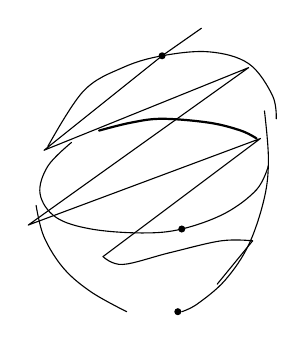
\begin{tikzpicture}[x=0.5mm,y=0.5mm,line cap=round,line join=round,font=\scriptsize]
\draw plot[smooth, tension=0.6] coordinates {(21,-45) (30,-31) (40,-25) (50,-22) (62,-21) (72,-24) (78,-32) (79,-38)};
\draw plot[smooth, tension=0.6] coordinates {(18,-60) (20,-68) (25,-76) (32,-82) (41,-87)};
\draw plot[smooth, tension=0.6] coordinates {(76,-36) (77,-48) (76,-58) (72,-70) (66,-79) (59,-85) (55,-87)};
\draw[thick] plot[smooth, tension=0.6] coordinates {(34,-41) (42,-39) (50,-38) (62,-39) (70,-41) (74,-43)};
\draw plot[smooth, tension=0.6] coordinates {(27,-44) (21,-50) (19,-57) (23,-63) (32,-66) (45,-67) (55,-66) (66,-62) (74,-56) (77,-50)};
\draw (60,-15) -- (50,-22) -- (20,-46) -- (72,-25) -- (16,-65) -- (75,-43) -- (35,-73);
\draw plot[smooth, tension=0.6] coordinates {(35,-73) (40,-75) (52,-72) (65,-69) (73,-69)};
\draw (73,-69) -- (64,-80);
\node[pt] at (50,-22) {};
\node[pt] at (55,-66) {};
\node[pt] at (54,-87) {};
\end{tikzpicture}
\end{document}
